\chapter{Standard DASH-MPEG}
\label{cha:rozdzial4}

\section{Wprowadzenie}
Poniższy rozdział opisuje standard Dynamic Adaptive Streaming over HTTP (DASH). Po zarysie historycznym i odniesieniu do pokrewnych technologii zaprezentowany zostaje podrozdział \ref{sec:dash-arch} zawierający zwięzły opis działania systemów wspierających strumieniowanie danych multimedialnych z wykorzystaniem DASH. Kolejne podrozdziały skupiają się na wybranych aspektach i funkcjonalnościach tego standardu takich jak hierarchiczna struktura modelu danych multimedialnych, synchronizacja strumieni oraz profile.

\section{Zarys historyczny}
Dynamic Adaptive Streaming over HTTP jest adaptacyjną techniką strumieniowania danych w sieciach komputerowych. Prace nad standardem prowadzone przez grupę MPEG rozpoczęły się w 2010 roku. W 2011 standard DASH pojawił się jako draft, a międzynarodowym standardem stał się w kwietniu 2012 dzięki publikacji ISO/IEC 23009-1:2012~\cite{ISO-IEC-DASH}. W lipcu 2013 wprowadzono do standardu poprawki.

DASH jest technologią spokrewnioną z Microsoft Smooth Streaming~\cite{MicroS}, Adobe Systems HTTP Dynamic Streaming~\cite{ADOBES} oraz Apple Inc. HTTP Live Streaming~\cite{APPLES}.

\section{Systemy implementujące DASH}
W podejściu stosowanym w standardzie DASH logika strumieniowania zostaje w całości przeniesiona na aplikację klienta. Rolę serwera DASH może pełnić zwykły serwer HTTP.
\label{sec:dash-arch}
\begin{figure}[h!]
	\centering
		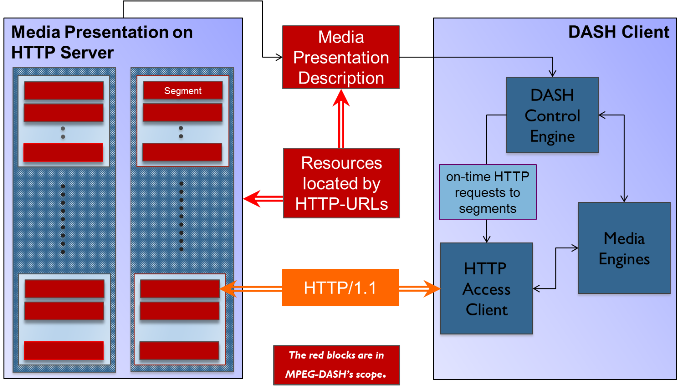
\includegraphics{dash}
	\caption{Standard MPEG-DASH i przykładowa architektura klienta DASH, źródło:~\cite{DASH}}
	\label{fig:dash}
\end{figure}
 Plik multimedialny, który będzie podlegał operacji strumieniowania, należy odpowiednio przygotować. Plik powinien być dostępny w kilku wersjach różniących się jakością (a co za tym idzie również wielkością).  Każda kopia powinna zostać podzielona na segmenty o równej długości. Na rysunku~\ref{fig:dash}~kopie pliku multimedialnego składają się z segmentów (czerwone prostokąty) umieszczonych na serwerze HTTP (lewa strona rysunku). Od długości segmentów zależeć będzie szybkość przystosowywania się aplikacji DASH do zmieniającej się przepustowości sieci. Tak przygotowane pliki należy opisać za pomocą XML w postaci dokumentu MPD (Media Presentation Description). Plik MPD zawiera adresy URL poszczególnych segmentów, informacje na temat kodowania danych, rozdzielczości oraz wymaganych przepustowości. Następnie MPD musi zostać dostarczony klientowi, który parsując jego zawartość otrzyma informacje na temat danych multimedialnych, które ma strumieniować. W trakcie strumieniowania, aplikacja klienta wybiera w sposób dynamiczny wersję danych i pobiera kolejny segment z pomocą protokołu HTTP. 
Standard DASH działa niezależnie od sposobu kodowania danych i jest łatwo implementowalny w Internecie. Dzięki wykorzystaniu protokołu HTTP może współpracować z istniejącą infrastrukturą w postaci filtrów, zapór, urządzeń NAT i cache~\cite{DASH}.

\section{Hierarchiczna struktura modelu danych}

Struktura modelu danych multimedialnych jest opisywana plikiem Media Presentation Description za pomocą języka XML i ma charakter hierarchiczny (zob.~rysunek~\ref{fig:mpd}). Lewy prostokąt symbolizuje plik MPD, który zawiera kilka elementów typu \textit{Period} (środkowy prostokąt na rysunku~\ref{fig:mpd}) oraz może zawierać informacje na temat profilu (zob.~\ref{sec:profile}). Elementy \textit{Period} reprezentują ciągłą część danych multimedialnych, które charakteryzują się takim samym zestawem parametrów. Do zestawu tych parametrów mogą należeć:
\begin{itemize}
	\item zbiór dostępnych wersji plików multimedialnych (zbiór różnych bitrate),
	\item wersje językowe (dla dźwięku),
	\item wersje językowe napisów,
	\item sposób kodowania danych,
	\item itd...
\end{itemize}
Parametry te pozostają niezmienne w pojedynczym elemencie \textit{Period}, ale mogą występować różnice pomiędzy różnymi elementami.
Wszystkie elementy \textit{Period} posiadają znacznik czasowy pozwalający na ustalenie ich kolejności, a dane znajdujące się w kolejnych elementach tworzą ciągły strumień danych multimedialnych.

\begin{figure}
	\centering
		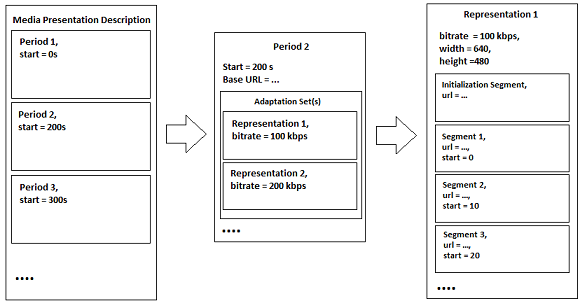
\includegraphics[width=\linewidth]{mpd}
	\caption{Struktura modelu danych, na podstawie~\cite{ISO-IEC-DASH}}
	\label{fig:mpd}
\end{figure}

Dane znajdujące się w pojedynczym elemencie \textit{Period} mogą zostać rozdzielone pomiędzy kilka elementów o nazwie \textit{Adaptation Set}. \textit{Adaptation Set} reprezentuje jedną lub kilka wersji komponentów danych multimedialnych. Przykładowo, możliwe jest odseparowanie danych video i audio poprzez przechowywanie ich w osobnych elementach \textit{Adaptation Set}. Dane tekstowe (napisy) również mogą zostać wydzielone w podobny sposób. Rezygnacja z multipleksacji danych pozwala na wprowadzenie kilku wersji danych (audio lub napisy dostępne w różnych wersjach językowych).

Każdy \textit{Adaptation Set} zawiera jeden lub kilka elementów typu \textit{Representation} (prawy prostokąt na rysunku~\ref{fig:mpd}). Typowo, dane multimedialne w poszczególnych elementach \textit{Representation} różnią się jakością, co w rezultacie wpływa na ich wielkość. W trakcie strumieniowania aplikacja klienta może wybierać pomiędzy różnymi wersjami danych na podstawie warunków panujących w sieci komputerowej (dostępna przepustowość, RTT\footnote{Round Trip Time - minimalny czas potrzebny na komunikację od nadawcy do odbiorcy i z powrotem.}) lub innych czynników.

Dane multimedialne w ramach \textit{Representation} mogą zostać podzielone na wiele części typu \textit{Segments}. Są to najmniejsze części danych jakie klient może pobrać za pomocą metody HTTP GET. Każdy \textit{Segment} ma określony czas trwania odpowiadający czasowi odtwarzania danych w nim zawartych oraz znacznik czasowy pozwalający na ustalenie ich właściwej kolejności. Elementy \textit{Segment} należące do tego samego \textit{Representation} zwykle mają porównywalny czas trwania.

\section{Osie czasu}

Standard DASH definiuje dwie osie czasu. Pierwsza z nich pozwala na synchronizację odtwarzania komponentów danych multimedialnych (audio/video/text). Metadane wymagane do synchronizacji można uzyskać z pliku MPD. Elementy \textit{Period} oraz \textit{Segment} posiadają atrybut ``start'' (zob. rysunek~\ref{fig:mpd}) pozwalający na określenie czasu w którym należy rozpocząć odtwarzanie zawieranych przez nie danych. W celu obliczenia bezwzględnego czasu w którym należy odtworzyć dany \textit{Segment} należy obliczyć sumę składającą się z wartości atrybutu ``start'' elemntu \textit{Period} do którego dany \textit{Segment} należy oraz wartości atrybutu ``start'' dla danego elementu typu \textit{Segment}.

Druga z osi czasu jest wykorzystywana do wskazywania aplikacji klienta okien czasowych w jakich dostępne są dane multimedialne. Okna te nazywane są ``Segment Availability Times''. Aplikacja klienta powinna sprawdzić dostępność danych (reprezentowanych przez \textit{Segment} posiadający własny URL) przed próbą ich pobrania. W przypadku modelów ``On Demand'' takich jak VoD\footnote{Video On Demand - usługa pozwalająca na odtwarzanie danych multimedialnych w wybranym przez użytkownika czasie, późniejszym niż czas emisji.} plik MPD nie ulega zmianie i okna czasowe dla wszystkich danych multimedialnych są jednakowe. Takie podejście pozwala klientowi na odtwarzanie danych znajdujących się w dowolnym miejscu na osi czasowej (możliwość wprowadzenia powtórek, przewijana transmisji do przodu lub do tyłu). Dla usług ``na żywo'', gdzie plik MPD jest aktualizowany w czasie działania aplikacji klienckich, okna czasowe charakteryzują się ograniczonym czasem życia związanym z położeniem danych multimedialnych na osi czasu. Użytkownik ma wtedy możliwość pobrania jedynie najnowszych danych (możliwość pobrania starszych danych jest limitowana wielkością okna czasowego - ``Segment Availability Time'').

\section{Model referencyjny klienta dla metryki DASH}

System zgodny z modelem referencyjnym dla metryki DASH posiada trzy punkty obserwacyjne (\textit{Observation Points}) w których dokonywane są pomiary dotyczące jakości transmisji danych multimedialnych i pracy aplikacji (zob. rysunek~\ref{fig:clientmodel}). 

\begin{figure}[h!]
	\centering
		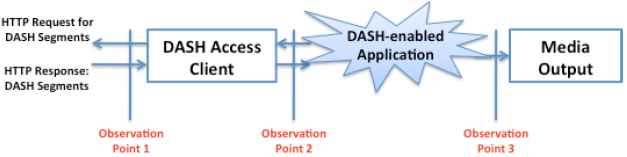
\includegraphics[width=\linewidth]{clientmodel}
	\caption{Model referencyjny klienta dla metryki DASH, źródło:~\cite{ISO-IEC-DASH}}
	\label{fig:clientmodel}
\end{figure}

Pierwszy punkt obserwacyjny znajduje się na styku połączenia sieciowego z komponentem aplikacji klienta odpowiedzialnym za zgłaszanie zapotrzebowania na dane i ich pobierania. W trakcie pracy tego komponentu monitorowane są:
\begin{itemize}
\item połączenia TCP - docelowy adres IP, czas rozpoczęcia, trwania i zakończenia połączenia,
\item sekwencja przesłanych wiadomości HTTP - czas transmisji, zawartość, połączenie TCP związane z transmisją,
\item odpowiedzi HTTP - czas otrzymania, zawartość nagłówka.
\end{itemize}

Drugi z punktów obserwacyjnych znajduje się pomiędzy komponentem odpowiedzialnym za pobieranie danych, a komponentem przetwarzającym otrzymane dane. Przetwarzanie danych może polegać na ich demultipleksowaniu (audio/video) lub dekodowaniu. W tym punkcie obserwacyjnym zbierane są informacje na temat kodowanych danych takie jak:
\begin{itemize}
\item typ danych - video, audio, tekst, itd...,
\item czas dostarczenia danych,
\item czas dekodowania danych,
\item poziom zapełnienia bufora dla pobieranych danych,
\item numer identyfikacyjny elementu \textit{Representation} z którego dane pochodzą.
\end{itemize} 

Ostatni z punktów obserwacyjnych znajduje się pomiędzy komponentem przetwarzającym dane oraz komponentem, który prezentuje przetworzone dane użytkownikowi.
\begin{itemize}
\item typ danych,
\item czas prezentowania danych wynikający z metadanych pliku MPD,
\item czas rzeczywisty prezentowania danych (timestamp),
\item numer identyfikacyjny elementu \textit{Representation} z którego dane pochodzą.
\end{itemize}

Tabele przedstawiające dokładną specyfikację metryk można znaleźć w specyfikacji standardu DASH-MPEG (\cite{ISO-IEC-DASH}) w dodatku D.

\section{Profile}
\label{sec:profile}

\section{Podsumowanie}
niedomagania i aspekty nad którymi warto się skupić.
